\documentclass[10pt]{article}
\usepackage[polish]{babel}
\usepackage[utf8]{inputenc}
\usepackage[T1]{fontenc}
\usepackage{amsmath}
\usepackage{amsfonts}
\usepackage{amssymb}
\usepackage[version=4]{mhchem}
\usepackage{stmaryrd}
\usepackage{multirow}
\usepackage{graphicx}
\usepackage[export]{adjustbox}
\graphicspath{ {./images/} }
\usepackage{fvextra, csquotes}

\title{EGZAMIN MATURALNY W ROKU SZKOLNYM 2016/2017 }

\author{ZASADY OCENIANIA ROZWIĄZAŃ ZADAŃ ARKUSZ MMA-P1}
\date{}


\newcommand\Varangle{\mathop{{<\!\!\!\!\!\text{\small)}}\:}\nolimits}

\begin{document}
\maketitle
FORMULA OD 2015\\
(,NOWA MATURA")



\section*{Zadania zamknięte}
Punkt przyznaje sie za wskazanie poprawnej odpowiedzi.\\
Zadanie 1. (0-1)

\begin{center}
\begin{tabular}{|l|l|c|c|}
\hline
\multicolumn{1}{|c|}{Wymagania ogólne} & \multicolumn{1}{|c|}{Wymagania szczegółowe} & \multicolumn{2}{|c|}{\begin{tabular}{c}
Poprawna \\
odp. (1 p.) \\
\end{tabular}} \\
\hline
\begin{tabular}{l}
II. Wykorzystanie \\
i interpretowanie \\
reprezentacji. \\
\end{tabular} & \begin{tabular}{l}
1. Liczby rzeczywiste. Zdający oblicza potegi \\
o wykładnikach wymiernych i stosuje prawa \\
działań na potęgach o wykładnikach \\
wymiernych (1.4). \\
\end{tabular} & \begin{tabular}{c}
Wersja \\
I \\
\end{tabular} & \begin{tabular}{c}
Wersja \\
II \\
\end{tabular} \\
\cline{3-4}
 & A & B &  \\
\hline
\end{tabular}
\end{center}

Zadanie 2. (0-1)\\
II. Wykorzystanie i interpretowanie reprezentacji.

\begin{center}
\begin{tabular}{|l}
1. Liczby rzeczywiste. Zdający posługuje \\
się wobliczeniach pierwiastkami dowolnego \\
stopnia i stosuje prawa działań na \\
pierwiastkach (1.3). \\
\end{tabular}
\end{center}

\begin{center}
\begin{tabular}{|c|c|}
\hline
\begin{tabular}{c}
Wersja \\
I \\
\end{tabular} & \begin{tabular}{c}
Wersja \\
II \\
\end{tabular} \\
\hline
C & D \\
\hline
\end{tabular}
\end{center}

\section*{Zadanie 3. (0-1)}
II. Wykorzystanie i interpretowanie reprezentacji.

\begin{enumerate}
  \item Liczby rzeczywiste. Zdający wykorzystuje\\
definicję logarytmu i stosuje w obliczeniach\\
wzory na logarytm iloczynu, logarytm ilorazu\\
i logarytm potęgi o wykładniku naturalnym\\
(1.6).
\end{enumerate}

\begin{center}
\begin{tabular}{|c|c|}
\hline
\begin{tabular}{c}
Wersja \\
I \\
\end{tabular} & \begin{tabular}{c}
Wersja \\
II \\
\end{tabular} \\
\hline
A & D \\
\hline
\end{tabular}
\end{center}

\section*{Zadanie 4. (0-1)}
\begin{center}
\begin{tabular}{|l|l|c|c|}
\hline
\begin{tabular}{l}
III. Modelowanie \\
matematyczne. \\
\end{tabular} & \begin{tabular}{l}
1. Liczby rzeczywiste. Zdający wykonuje \\
obliczenia procentowe, oblicza podatki, zysk \\
z lokat (1.9). \\
\end{tabular} & \begin{tabular}{c}
Wersja \\
$\mathbf{I}$ \\
\end{tabular} & \begin{tabular}{c}
Wersja \\
II \\
\end{tabular} \\
\cline { 3 - 4 }
 &  & $\mathbf{A}$ & $\mathbf{B}$ \\
\hline
\end{tabular}
\end{center}

\section*{Zadanie 5. (0-1)}
\begin{center}
\begin{tabular}{|l|l|c|c|}
\hline
\begin{tabular}{l}
II. Wykorzystanie \\
i interpretowanie \\
reprezentacji. \\
\end{tabular} & \begin{tabular}{l}
3. Równania i nierówności. Zdający \\
rozwiązuje równania kwadratowe z jedną \\
niewiadomą (3.4). \\
\end{tabular} & \begin{tabular}{c}
Wersja \\
$\mathbf{I}$ \\
\end{tabular} & \begin{tabular}{c}
Wersja \\
II \\
\end{tabular} \\
\cline { 3 - 4 }
 &  & $\mathbf{C}$ & $\mathbf{D}$ \\
\hline
\end{tabular}
\end{center}

Zadanie 6. (0-1)

\begin{center}
\begin{tabular}{|l|l|c|c|}
\hline
\multirow{2}{*}{\begin{tabular}{l}
I. Wykorzystanie \\
i tworzenie informacji. \\
\end{tabular}} & \begin{tabular}{l}
3. Równania i nierówności. Zdający sprawdza, \\
czy dana liczba rzeczywista jest rozwiązaniem \\
równania lub nierówności (3.1). \\
\end{tabular} & \begin{tabular}{c}
Wersja \\
I \\
\end{tabular} & \begin{tabular}{c}
Wersja \\
II \\
\end{tabular} \\
\cline{3-4}
 & D & C &  \\
\hline
\end{tabular}
\end{center}

Zadanie 7. (0-1)\\
$\left.\begin{array}{|l|l|c|c|}\hline \text { I. Wykorzystanie } \\ \text { i tworzenie informacji }\end{array} \begin{array}{l}\text { 3. Równania i nierówności. Zdający } \\ \text { rozwiązuje nierówności pierwszego stopnia } \\ \text { z jedną niewiadomą (3.3). }\end{array} \begin{array}{c}\text { Wersja } \\ \mathbf{I}\end{array} \begin{array}{c}\text { Wersja } \\ \text { II }\end{array}\right]$

Zadanie 8. (0-1)\\
$\left.\begin{array}{|l|l|c|c|}\hline \text { I. Wykorzystanie } \\ \text { i tworzenie informacji. }\end{array} \begin{array}{l}\text { 3. Równania i nierówności. Zdający korzysta } \\ \text { z własności iloczynu przy rozwiązywaniu } \\ \text { równań typu } x(x+1)(x-7)=0(3.7) .\end{array} \begin{array}{c}\text { Wersja } \\ \text { I }\end{array} \begin{array}{c}\text { Wersja } \\ \text { II }\end{array}\right]$

\section*{Zadanie 9. (0-1)}
$\left.$\textbackslash begin\{tabular\}\{|l|l|c|c|\}\\
\textbackslash hline II. Wykorzystanie \\
\\
i interpretowanie \\
\\
reprezentacji.

 \begin{tabular}{l}
\end{tabular}

\begin{enumerate}
  \setcounter{enumi}{3}
  \item Funkcje. Zdający oblicza ze wzoru wartość \\
\\
funkcji dla danego argumentu. Posługuje się \\
\\
poznanymi metodami rozwiązywania równań \\
\\
do obliczenia, dla jakiego argumentu funkcja \\
\\
przyjmuje daną wartość (4.2).
\end{enumerate}

 \begin{tabular}{c}
\end{tabular}

Wersja \\
\\
I

 \begin{tabular}{c}
\end{tabular}

Wersja \\
\\
II\\
\textbackslash end\{tabular\} \textbackslash right\textbackslash rvert,

Zadanie 10. (0-1)

\begin{center}
\begin{tabular}{|l|l|c|c|}
\hline
I. Wykorzystanie &  &  &  \\
i tworzenie informacji & \begin{tabular}{l}
4. Funkcje. Zdajaccy interpretuje \\
współczynniki występujące we wzorze funkcji \\
kwadratowej w postaci kanonicznej, w postaci \\
ogólnej i w postaci iloczynowej (o ile istnieje) \\
(4.10). \\
\end{tabular} & \begin{tabular}{c}
Wersja \\
I \\
\end{tabular} & \begin{tabular}{c}
Wersja \\
II \\
\end{tabular} \\
\cline{4-4}
 & C & A &  \\
\hline
\end{tabular}
\end{center}

\section*{Zadanie 11. (0-1)}
\begin{center}
\begin{tabular}{|l|l|c|c|}
\hline
\multirow{2}{*}{\begin{tabular}{l}
II. Wykorzystanie \\
i interpretowanie \\
reprezentacji. \\
\end{tabular}} & 4. Funkcje. Zdający szkicuje wykresy funkcji & \begin{tabular}{c}
Wersja \\
I \\
\end{tabular} & \begin{tabular}{c}
Wersja \\
II \\
\end{tabular} \\
\cline { 3 - 4 }
 & wykładniczych dla róznych podstaw (4.14). & D & B \\
\hline
\end{tabular}
\end{center}

Zadanie 12. (0-1)

\begin{center}
\begin{tabular}{|l|l|c|c|}
\hline
\begin{tabular}{l}
III. Modelowanie \\
matematyczne. \\
\end{tabular} & \begin{tabular}{l}
5. Ciągi. Zdający stosuje wzór na $n$-ty wyraz \\
i na sumę $n$ początkowych wyrazów ciągu \\
arytmetycznego (5.3). \\
\end{tabular} & \begin{tabular}{c}
Wersja \\
I \\
\end{tabular} & \begin{tabular}{c}
Wersja \\
II \\
\end{tabular} \\
\cline { 3 - 4 }
 & B & C &  \\
\hline
\end{tabular}
\end{center}

Zadanie 13. (0-1)

\begin{center}
\begin{tabular}{|l|l|c|c|}
\hline
\begin{tabular}{l}
III. Modelowanie \\
matematyczne. \\
\end{tabular} & \begin{tabular}{l}
5. Ciągi. Zdajaccy stosuje wzór na $n$-ty wyraz \\
i na sumę $n$ początkowych wyrazów ciągu \\
geometrycznego (5.4). \\
\end{tabular} & \begin{tabular}{c}
Wersja \\
I \\
\end{tabular} & \begin{tabular}{c}
Wersja \\
II \\
\end{tabular} \\
\cline { 3 - 4 }
 & A & B &  \\
\hline
\end{tabular}
\end{center}

Zadanie 14. (0-1)

\begin{center}
\begin{tabular}{|l|l|c|c|}
\hline
\begin{tabular}{l}
II. Wykorzystanie \\
i interpretowanie \\
reprezentacji. \\
\end{tabular} & \begin{tabular}{l}
6. Trygonometria. Zdajacy stosuje proste \\
zależności między funkcjami \\
trygonometrycznymi: $\sin ^{2} \alpha+\cos ^{2} \alpha=1$, \\
$\operatorname{tg} \alpha=\frac{\sin \alpha}{\cos \alpha}$ oraz $\sin \left(90^{\circ}-\alpha\right)=\cos \alpha(6.4)$. \\
\end{tabular} & \begin{tabular}{c}
Wersja \\
I \\
\end{tabular} & \begin{tabular}{c}
Wersja \\
II \\
\end{tabular} \\
\cline { 3 - 4 }
 & B & C &  \\
\hline
\end{tabular}
\end{center}

\section*{Zadanie 15. (0-1)}
$\left.$\textbackslash begin\{tabular\}\{|l|l|c|c|\}\\
\textbackslash hline IV. Użycie i tworzenie \\
\\
strategii.

 \begin{tabular}{l}
\end{tabular}

\begin{enumerate}
  \setcounter{enumi}{6}
  \item Planimetria. Zdający stosuje zależności \\
\\
między kątem środkowym i kątem wpisanym \\
\\
(7.1).
\end{enumerate}

 \begin{tabular}{c}
\end{tabular}

Wersja \\
\\
I

 \begin{tabular}{c}
\end{tabular}

Wersja \\
\\
II\\
\textbackslash end\{tabular\} \textbackslash right\textbackslash rvert,

Zadanie 16. (0-1)

\begin{center}
\begin{tabular}{|l|l|c|c|}
\hline
\begin{tabular}{l}
I. Wykorzystanie \\
i tworzenie informacji. \\
\end{tabular} & \begin{tabular}{l}
7. Planimetria. Zdający rozpoznaje trójkąty \\
podobne i wykorzystuje cechy podobieństwa \\
trójkątów (7.3). \\
\end{tabular} & \begin{tabular}{c}
Wersja \\
I \\
\end{tabular} & \begin{tabular}{c}
Wersja \\
II \\
\end{tabular} \\
\cline { 3 - 4 }
 & B & A &  \\
\hline
\end{tabular}
\end{center}

\section*{Zadanie 17. (0-1)}
III. Modelowanie matematyczne.

\begin{center}
\begin{tabular}{|l|l|}
7. Planimetria. Zdający korzysta z własności \\
funkcji trygonometrycznych w łatwych \\
obliczeniach geometrycznych, w tym ze \\
wzoru na pole trójkąta ostrokątnego o danych \\
dwóch bokach i kącie między nimi (7.4). \\
\end{tabular}
\end{center}

\begin{center}
\begin{tabular}{|c|c|}
\hline
\begin{tabular}{c}
Wersja \\
I \\
\end{tabular} & \begin{tabular}{c}
Wersja \\
II \\
\end{tabular} \\
\hline
C & D \\
\hline
\end{tabular}
\end{center}

Zadanie 18. (0-1)

\begin{center}
\begin{tabular}{|c|c|c|c|}
\hline
\multirow[t]{2}{*}{II. Wykorzystanie i interpretowanie reprezentacji.} & 6. Trygonometria. Zdający wykorzystuje definicje i wyznacza wartości funkcji sinus, & Wersja I & Wersja II \\
\hline
 & \( 180^{\circ}(6.1) \) & B & C \\
\hline
\end{tabular}
\end{center}

Zadanie 19. (0-1)

\begin{center}
\begin{tabular}{|l|l|c|c|}
\hline
\multirow{2}{*}{\begin{tabular}{l}
II. Wykorzystanie \\
i interpretowanie \\
reprezentacji. \\
\end{tabular}} & \begin{tabular}{l}
8. Geometria na płaszczyźnie kartezjańskiej. \\
Zdający bada równoległość i prostopadłość \\
prostych na podstawie ich równań \\
kierunkowych (8.2). \\
\end{tabular} & \begin{tabular}{c}
Wersja \\
I \\
\end{tabular} & \begin{tabular}{c}
Wersja \\
II \\
\end{tabular} \\
\cline { 3 - 4 }
 & D & A &  \\
\hline
\end{tabular}
\end{center}

Zadanie 20. (0-1)

\begin{center}
\begin{tabular}{|l|l|c|c|}
\hline
\begin{tabular}{l}
II. Wykorzystanie \\
i interpretowanie \\
reprezentacji. \\
\end{tabular} & \begin{tabular}{l}
8. Geometria na płaszczyźnie kartezjańskiej. \\
Zdajạcy oblicza odległość dwóch punktów \\
(8.6). \\
\end{tabular} & \begin{tabular}{c}
Wersja \\
I \\
\end{tabular} & \begin{tabular}{c}
Wersja \\
II \\
\end{tabular} \\
\cline{3-4}
 & A & C &  \\
\hline
\end{tabular}
\end{center}

Zadanie 21. (0-1)

\begin{center}
\begin{tabular}{|c|c|c|c|}
\hline
\multirow[b]{2}{*}{II. Wykorzystanie i interpretowanie reprezentacji.} & G11. Bryły. Zdający oblicza pole powierzchni i objętość graniastosłupa prostego (G11.2). & Wersja I & \begin{tabular}{l}
Wersja \\
II \\
\end{tabular} \\
\hline
 & 3. Równania i nierówności. Zdający rozwiązuje równania kwadratowe z jedną niewiadomą (3.4). & A & B \\
\hline
\end{tabular}
\end{center}

Zadanie 22. (0-1)

\begin{center}
\begin{tabular}{|l|l|c|c|}
\hline
\multirow{2}{*}{\begin{tabular}{l}
II. Wykorzystanie \\
i interpretowanie \\
reprezentacji. \\
\end{tabular}} & \begin{tabular}{l}
9. Stereometria. Zdający rozpoznaje \\
w walcach i w stożkach kąt między odcinkami \\
oraz kąt między odcinkami i płaszczyznami \\
(9.3). \\
\end{tabular} & \begin{tabular}{c}
Wersja \\
I \\
\end{tabular} & \begin{tabular}{c}
Wersja \\
II \\
\end{tabular} \\
\cline{3-4}
 & B & C &  \\
\hline
\end{tabular}
\end{center}

Zadanie 23. (0-1)

\begin{center}
\begin{tabular}{|l|l|c|c|}
\hline
\multirow{2}{*}{\begin{tabular}{l}
II. Wykorzystanie \\
i interpretowanie \\
reprezentacji. \\
\end{tabular}} & \begin{tabular}{l}
G11. Bryły. Zdający oblicza pole powierzchni \\
i objętość stożka (G11.2). \\
\end{tabular} & \begin{tabular}{c}
Wersja \\
I \\
\end{tabular} & \begin{tabular}{c}
Wersja \\
II \\
\end{tabular} \\
\cline { 3 - 4 }
 & D & A &  \\
\hline
\end{tabular}
\end{center}

Zadanie 24. (0-1)

\begin{center}
\begin{tabular}{|l|l|c|c|}
\hline
\multirow{2}{l}{\begin{tabular}{l}
II. Wykorzystanie \\
i interpretowanie \\
reprezentacji. \\
\end{tabular}} & \begin{tabular}{l}
G9. Statystyka opisowa i wprowadzenie do \\
rachunku prawdopodobieństwa. Zdajacy \\
wyznacza średnią arytmetyczną i medianę \\
zestawu danych (G9.4). \\
\end{tabular} & \begin{tabular}{c}
Wersja \\
I \\
\end{tabular} & \begin{tabular}{c}
Wersja \\
II \\
\end{tabular} \\
\cline { 3 - 4 }
 & D & B &  \\
\hline
\end{tabular}
\end{center}

Zadanie 25. (0-1)

\begin{center}
\begin{tabular}{|l|l|c|c|}
\hline
 & \begin{tabular}{l}
10. Elementy statystyki opisowej. Teoria \\
prawdopodobieństwa i kombinatoryka. \\
III. Modelowanie \\
matematyczne. \\
\end{tabular} & \begin{tabular}{l}
Zdający oblicza prawdopodobieństwa \\
w prostych sytuacjach, stosując klasyczną \\
definicję prawdopodobienstwa (10.3). \\
\end{tabular} & \begin{tabular}{c}
Wersja \\
II \\
\end{tabular} \\
\cline{3-4}
 & B & C &  \\
\hline
\end{tabular}
\end{center}

\section*{Ogólne zasady oceniania zadań otwartych}
Uwaga: Akceptowane sa wszystkie odpowiedzi merytorycznie poprawne i spetniajace warunki zadania.

\section*{Zadanie 26. (0-2)}
\begin{center}
\begin{tabular}{|l|l|}
\hline
\begin{tabular}{l}
II. Wykorzystanie \\
i interpretowanie \\
reprezentacji. \\
\end{tabular} & \begin{tabular}{l}
3. Równania i nierówności. Zdający rozwiązuje nierówności \\
kwadratowe $z$ jedną niewiadomą (3.5). \\
\end{tabular} \\
\hline
\end{tabular}
\end{center}

\section*{Przykładowe rozwiązanie}
Rozwiązanie nierówności kwadratowej składa się z dwóch etapów.\\
Pierwszy etap rozwiązania polega na wyznaczeniu pierwiastków trójmianu kwadratowego $8 x^{2}-72 x$.\\
Znajdujemy pierwiastki trójmianu kwadratowego $8 x^{2}-72 x$ :

\begin{itemize}
  \item podajemy je bezpośrednio, np. zapisując $x_{1}=0, x_{2}=9$ lub zaznaczając pierwiastki trójmianu na wykresie\\
albo
  \item obliczamy wyróżnik tego trójmianu, a następnie stosujemy wzory na pierwiastki:
\end{itemize}

$$
\Delta=72^{2}, x_{1}=\frac{72-72}{16}=0, x_{2}=\frac{72+72}{16}=9 .
$$

Drugi etap rozwiązania polega na wyznaczeniu zbioru rozwiązań nierówności $8 x^{2}-72 x \leq 0$. Podajemy zbiór rozwiązań nierówności: $0 \leq x \leq 9$ lub $\langle 0,9\rangle$ lub $x \in\langle 0,9\rangle$ np. odczytując go ze szkicu wykresu funkcji $f(x)=8 x^{2}-72 x$.\\
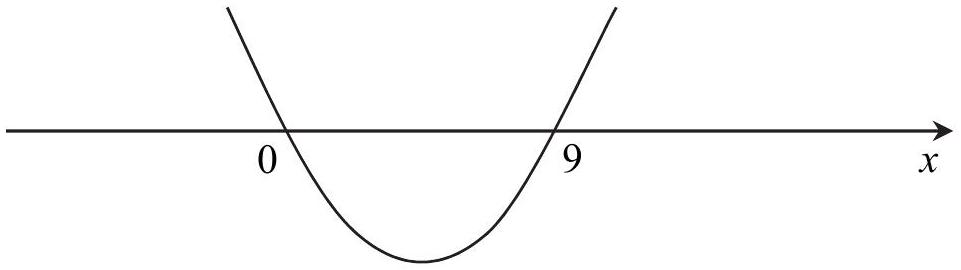
\includegraphics[max width=\textwidth, center]{2025_02_07_e35f706dbfcfb4be75cfg-06}

\section*{Schemat punktowania}
Zdający otrzymuje 1 p. gdy:

\begin{itemize}
  \item zrealizuje pierwszy etap rozwiązania i na tym zakończy lub błędnie zapisze zbiór rozwiązań nierówności, np.
  \item obliczy lub poda pierwiastki trójmianu kwadratowego $x_{1}=0$ i $x_{2}=9$ i na tym zakończy lub błędnie zapisze zbiór rozwiązań nierówności,
  \item zaznaczy na wykresie miejsca zerowe funkcji $f(x)=8 x^{2}-72 x$ i na tym zakończy lub błędnie zapisze zbiór rozwiązań nierówności\\
albo
  \item realizując pierwszy etap błędnie wyznaczy pierwiastki (ale otrzyma dwa różne pierwiastki) i konsekwentnie do tego rozwiąże nierówność, np. popełni błąd\\
rachunkowy przy obliczaniu wyróżnika lub pierwiastków trójmianu kwadratowego i konsekwentnie do popełnionego błędu rozwiąże nierówność.
\end{itemize}

\begin{verbatim}
Zdający otrzymuje
2 p.
gdy:
    - poda zbiór rozwiązań nierówności: 0\leqx\leq9 lub <0,9\rangle lub }x\in\langle0,9
albo
- poda zbiór rozwiązań nierówności w postaci graficznej z poprawnie zaznaczonymi końcami przedziałów
\end{verbatim}

\begin{center}
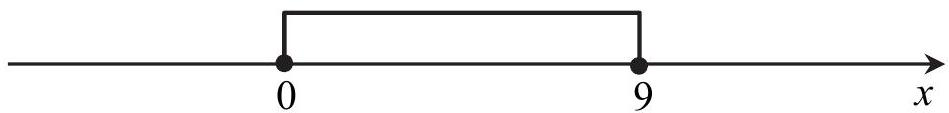
\includegraphics[max width=\textwidth]{2025_02_07_e35f706dbfcfb4be75cfg-07}
\end{center}

\section*{Uwagi}
\begin{enumerate}
  \item Jeżeli zdający dzieli obie strony nierówności przez $x$, bez podania stosownych założeń, to otrzymuje $\mathbf{0}$ punktów za całe rozwiązanie.
  \item Jeżeli zdający podaje pierwiastki bez związku z trójmianem kwadratowym z zadania, to oznacza, że nie podjął realizacji 1. etapu rozwiązania i w konsekwencji otrzymuje 0 punktów za całe rozwiązanie.
  \item Jeśli zdający wyznacza ujemną deltę trójmianu kwadratowego, to otrzymuje $\mathbf{0}$ punktów za całe rozwiązanie.
\end{enumerate}

Kryteria oceniania uwzględniające specyficzne trudności w uczeniu się matematyki

\begin{enumerate}
  \item Akceptujemy sytuację, gdy zdający poprawnie obliczy lub poda pierwiastki trójmianu $x_{1}=0$ i $x_{2}=9$ i zapisze, np. $x \in\langle-9,0\rangle$, popełniając tym samym błąd przy przepisywaniu jednego z pierwiastków, to za takie rozwiązanie otrzymuje 2 punkty.
  \item Jeśli zdający pomyli porządek liczb na osi liczbowej, np. zapisze zbiór rozwiązań nierówności w postaci $x \in\langle 9,0\rangle$, to przyznajemy 2 punkty.\\
V. Rozumowanie i argumentacja.
  \item Liczby rzeczywiste. Zdający wykorzystuje podstawowe własności potęg (1.5).
\end{enumerate}

\section*{Przykładowe rozwiązanie}
Wyłączamy wspólny czynnik przed nawias $4^{2017}\left(1+4+4^{2}+4^{3}\right)$. Doprowadzamy liczbę do postaci $4^{2017} \cdot 5 \cdot 17$. Wnioskujemy, że dana liczba jest podzielna przez 17 .

\section*{Schemat punktowania}
Zdający otrzymuje $\qquad$ 1 p. gdy zapisze liczbę $4^{2017}+4^{2018}+4^{2019}+4^{2020}$ w postaci iloczynu, w którym jeden z czynników jest potęgą $4^{k}$, gdzie $1985 \leq k \leq 2017$, np. $4^{2017}\left(1+4+4^{2}+4^{3}\right)$ i na tym poprzestanie lub dalej popełnia błędy.\\
Zdający otrzymuje gdy przeprowadzi poprawny dowód.

Zadanie 28. (0-2)\\
V. Rozumowanie i argumentacja.

\begin{displayquote}
G10. Figury płaskie. Zdający korzysta z faktu, że styczna do okręgu jest prostopadła do promienia poprowadzonego do punktu styczności (G10.3).\\
SP9. Wielokąty, koła, okręgi. Zdający stosuje twierdzenie o sumie katów trójkąta (SP9.3).
\end{displayquote}

\section*{Przykładowe rozwiązania}
I sposób\\
Przyjmijmy oznaczenia jak na rysunku.\\
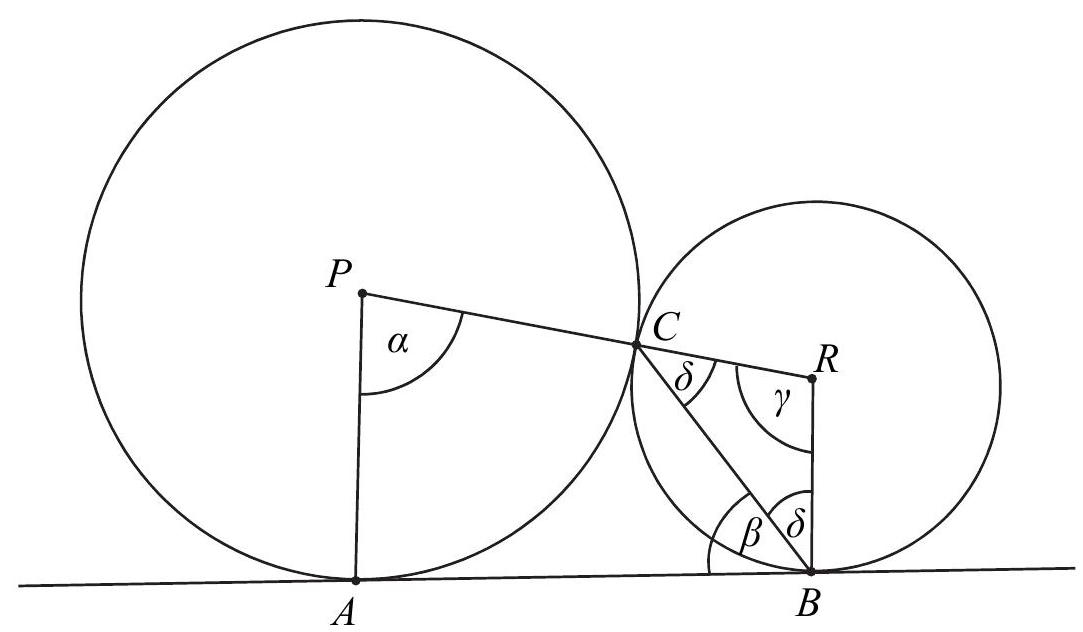
\includegraphics[max width=\textwidth, center]{2025_02_07_e35f706dbfcfb4be75cfg-08}

Prosta $A B$ jest styczna w punkcie $B$ do okręgu o środku $R$, więc $|\Varangle A B R|=90^{\circ}$. Stąd

$$
\delta=|\Varangle C B R|=90^{\circ}-\beta .
$$

Trójkąt $B R C$ jest równoramienny, więc

$$
|\Varangle B C R|=\delta=90^{\circ}-\beta .
$$

Zatem

$$
|\Varangle B R C|=\gamma=180^{\circ}-2\left(90^{\circ}-\beta\right)=2 \beta .
$$

Suma miar kątów czworokąta $A B R P$ jest równa $360^{\circ},|\Varangle P A B|=90^{\circ}$, więc

$$
|\Varangle P A B|+|\Varangle A B R|+|\Varangle B R P|+|\Varangle R P A|=360^{\circ},
$$

czyli

$$
\begin{gathered}
90^{\circ}+90^{\circ}+2 \beta+\alpha=360^{\circ}, \\
\alpha+2 \beta=180^{\circ}, \\
\alpha=180^{\circ}-2 \beta .
\end{gathered}
$$

To kończy dowód.

II sposób\\
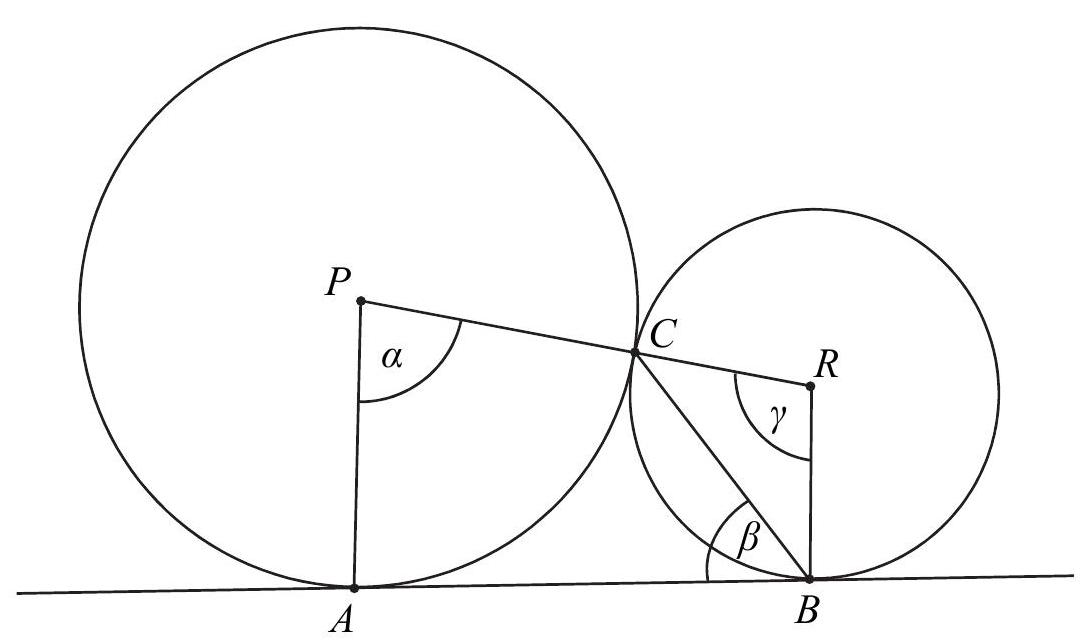
\includegraphics[max width=\textwidth, center]{2025_02_07_e35f706dbfcfb4be75cfg-09}

Z twierdzenia o kącie między styczną a cięciwą wynika, że $|\Varangle B R C|=\gamma=2 \beta$.\\
Ponieważ $|\Varangle A B R|=90^{\circ}$ i $|\Varangle P A B|=90^{\circ}$, więc czworokąt $A B R P$ jest trapezem o podstawach $A P$ i $B R$. Suma miar kątów przy ramieniu trapezu jest równa $180^{\circ}$, więc

$$
\begin{gathered}
\alpha+\gamma=180^{\circ}, \\
\alpha+2 \beta=180^{\circ} .
\end{gathered}
$$

Stąd $\alpha=180^{\circ}-2 \beta$. To kończy dowód.

\section*{III sposób}
\begin{center}
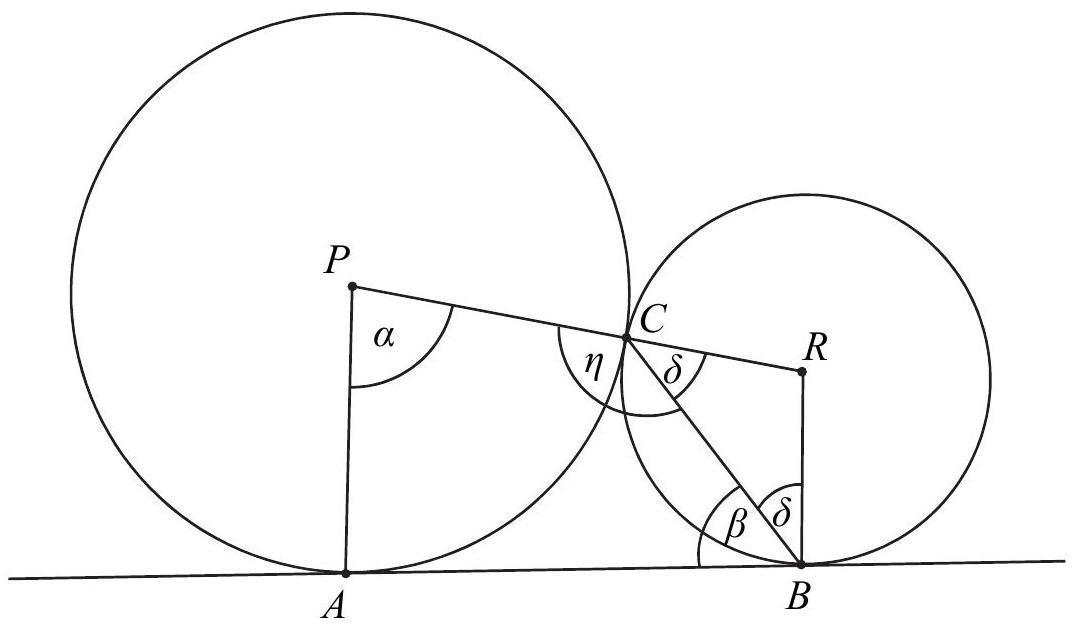
\includegraphics[max width=\textwidth]{2025_02_07_e35f706dbfcfb4be75cfg-10(1)}
\end{center}

Prosta $A B$ jest styczna w punkcie $B$ do okręgu o środku $R$, więc $|\Varangle A B R|=90^{\circ}$. Stąd

$$
\delta=90^{\circ}-\beta
$$

Trójkąt $B R C$ jest równoramienny, więc

$$
|\Varangle B C R|=\delta=90^{\circ}-\beta .
$$

Kąty $B C R$ i $P C B$ są przyległe, więc

$$
\eta=180^{\circ}-|\Varangle B C R|=180^{\circ}-\left(90^{\circ}-\beta\right)=90^{\circ}+\beta .
$$

Suma miar kątów czworokąta $A B C P$ jest równa $360^{\circ},|\Varangle P A B|=90^{\circ}$, więc

$$
|\Varangle P A B|+|\Varangle A B R|+|\Varangle B C P|+|\Varangle C P A|=360^{\circ},
$$

czyli

$$
\begin{gathered}
90^{\circ}+\beta+\eta+\alpha=360^{\circ}, \\
90^{\circ}+\beta+\left(90^{\circ}+\beta\right)+\alpha=360^{\circ}, \\
\alpha=180^{\circ}-2 \beta .
\end{gathered}
$$

To kończy dowód.

IV sposób\\
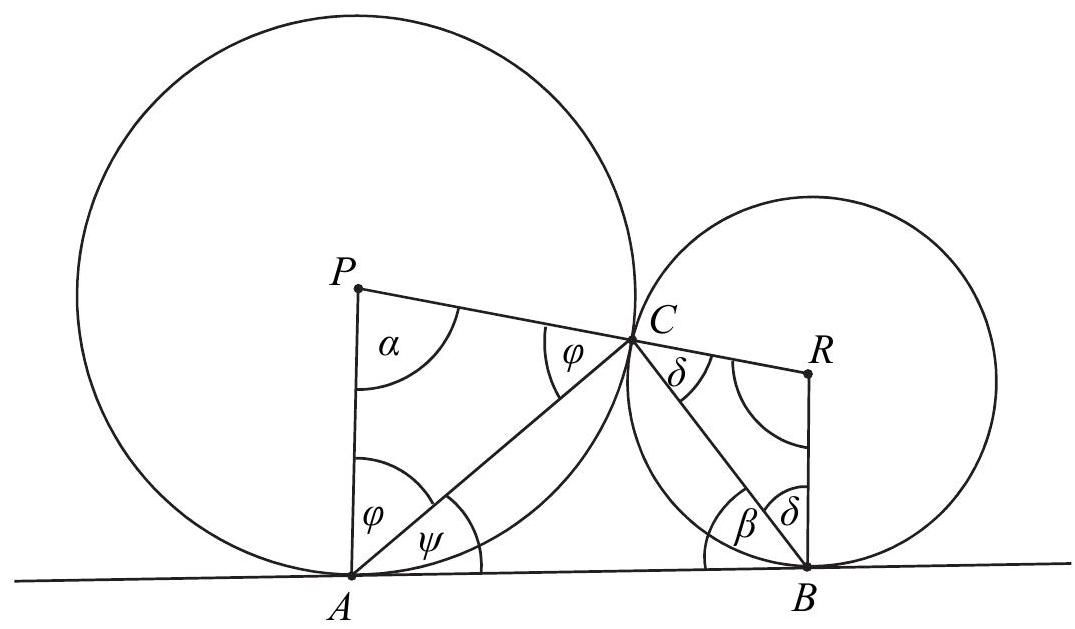
\includegraphics[max width=\textwidth, center]{2025_02_07_e35f706dbfcfb4be75cfg-10}

Prosta $A B$ jest styczna w punkcie $B$ do okręgu o środku $R$, więc $|\Varangle A B R|=90^{\circ}$.

Stąd $\delta=90^{\circ}-\beta$.\\
Trójkąt $B R C$ jest równoramienny, więc

$$
|\Varangle B C R|=\delta=90^{\circ}-\beta .
$$

Trójkąt $P A C$ jest równoramienny, więc

$$
|\Varangle P A C|=|\Varangle P C A|=\varphi=\frac{180^{\circ}-\alpha}{2}=90^{\circ}-\frac{\alpha}{2} .
$$

Prosta $A B$ jest styczna w punkcie $A$ do okręgu o środku $P$, więc $|\Varangle P A B|=90^{\circ}$. Stąd

$$
|\Varangle C A B|=\psi=90^{\circ}-\varphi=90^{\circ}-\left(90^{\circ}-\frac{\alpha}{2}\right)=\frac{\alpha}{2} .
$$

Miara kąta $A C B$ w trójkącie $A B C$ jest równa

$$
|\Varangle A C B|=180^{\circ}-\beta-\psi=180^{\circ}-\beta-\frac{\alpha}{2} .
$$

Suma miar kątów $P C A, A C B$ i $B C R$ jest równa $180^{\circ}$, więc

$$
\begin{gathered}
|\Varangle P C A|+|\Varangle A C B|+|\Varangle B C R|=180^{\circ}, \\
\varphi+\left(180^{\circ}-\beta-\frac{\alpha}{2}\right)+\delta=180^{\circ}, \\
90^{\circ}-\frac{\alpha}{2}+\left(180^{\circ}-\beta-\frac{\alpha}{2}\right)+90^{\circ}-\beta=180^{\circ}, \\
\alpha=180^{\circ}-2 \beta .
\end{gathered}
$$

To kończy dowód.\\
V sposób\\
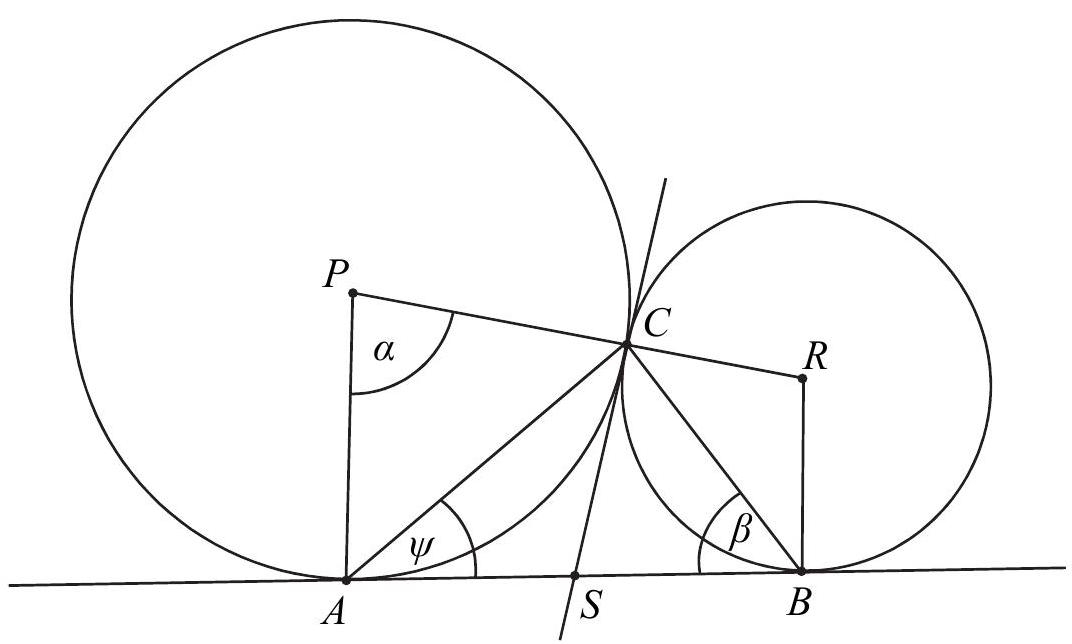
\includegraphics[max width=\textwidth, center]{2025_02_07_e35f706dbfcfb4be75cfg-11}

Poprowadźmy przez punkt $C$ wspólną styczną do obu okręgów. Niech $S$ oznacza punkt jej przecięcia z prostą $A B$.\\
Z twierdzenia o kącie między styczną a cięciwą wynika, że

$$
\psi=\frac{\alpha}{2} .
$$

Z twierdzenia o odcinkach stycznych wynika, że $|A S|=|C S|=|B S|$. Stąd wynika, że $S$ jest środkiem okręgu opisanego na trójkącie $A B C$. Odcinek $A B$ jest średnicą tego okręgu, więc trójkąt $A B C$ jest prostokątny. Suma miar jego kątów ostrych jest równa $90^{\circ}$, czyli

$$
\begin{gathered}
\beta+\psi=90^{\circ} . \\
\beta+\frac{\alpha}{2}=90^{\circ} \\
\alpha=180^{\circ}-2 \beta
\end{gathered}
$$

To kończy dowód.

\section*{Schemat punktowania}
Zdający otrzymuje\\
gdy zapisze układ warunków wystarczający do udowodnienia równości $\alpha=180^{\circ}-2 \beta$, np.:

\begin{itemize}
  \item $\delta=90^{\circ}-\beta$ i $2 \delta+\gamma=180^{\circ}$ i $\alpha+\gamma+90^{\circ}+90^{\circ}=360^{\circ}$\\
lub
  \item $\gamma=2 \beta$ i $\alpha+\gamma=180^{\circ}$,\\
lub
  \item $\delta=90^{\circ}-\beta$ i $\eta=180^{\circ}-\delta$ i $90^{\circ}+\beta+\eta+\alpha=360^{\circ}$,\\
lub
  \item $\delta=90^{\circ}-\beta$ i $\varphi=90^{\circ}-\frac{\alpha}{2}$ i $\psi=90^{\circ}-\varphi$ i $180^{\circ}-(\beta+\psi)=180^{\circ}-(\varphi+\delta)$,\\
lub
  \item $\beta+\psi=90^{\circ}$ i $\psi=\frac{\alpha}{2}$\\
i na tym zakończy lub dalej popełnia błędy.\\
Zdający otrzymuje 2 p.\\
gdy przeprowadzi pełne rozumowanie.
\end{itemize}

Zadanie 29. (0-4)\\
IV. Użycie i tworzenie strategii.\\
4. Funkcje. Zdający wyznacza wzór funkcji kwadratowej na podstawie pewnych informacji o tej funkcji lub o jej wykresie (4.9).

\section*{Przykładowe rozwiązania}
I sposób\\
Ponieważ $f(-6)=f(0)=\frac{3}{2}$, stąd wartość $p=\frac{-6+0}{2}=-3$.\\
Zatem $f(x)=a(x-p)^{2}+q$ dla $p=-3$ i $q=6$.\\
Obliczamy współczynnik $a$. Wiemy, że $f(0)=\frac{3}{2}$, zatem

$$
\begin{gathered}
a(0+3)^{2}+6=\frac{3}{2}, \\
9 a=-\frac{9}{2}, \\
a=-\frac{1}{2} .
\end{gathered}
$$

Odpowiedź: $a=-\frac{1}{2}$.\\
II sposób\\
Z treści zadania wynika, że $f(-6)=f(0)=\frac{3}{2}$ :

$$
\left\{\begin{array}{l}
a(-6)^{2}+b(-6)+c=\frac{3}{2} \\
a \cdot 0-b \cdot 0+c=\frac{3}{2}
\end{array},\left\{\begin{array}{l}
36 a-6 b+c=\frac{3}{2} \\
c=\frac{3}{2}
\end{array},\left\{\begin{array}{l}
b=6 a \\
c=\frac{3}{2}
\end{array} .\right.\right.\right.
$$

Obliczamy pierwszą współrzędną wierzchołka:

$$
p=-\frac{b}{2 a}=-\frac{6 a}{2 a}=-3 .
$$

Stąd wynika, że $f(-3)=6$ i $f(x)=a x^{2}+6 a x+\frac{3}{2}$. Obliczamy współczynnik $a$

$$
\begin{gathered}
a(-3)^{2}+6 a \cdot(-3)+\frac{3}{2}=6, \\
-9 a=\frac{9}{2}, \\
a=-\frac{1}{2} .
\end{gathered}
$$

\section*{Schemat punktowania}
Rozwiązanie, w którym postęp jest wprawdzie niewielki, ale konieczny na drodze do pełnego rozwiązania\\
Zdający

\begin{itemize}
  \item obliczy pierwszą współrzędną wierzchołka: np. $p=\frac{-6+0}{2}=-3$\\
albo
  \item zapisze układ dwóch równań, np.: $\left\{\begin{array}{l}a(-6)^{2}+b(-6)+c=\frac{3}{2} \\ a \cdot 0-b \cdot 0+c=\frac{3}{2},\end{array}\right.$\\
albo
  \item zapisze wzór funkcji $f$ w postaci kanonicznej $f(x)=a(x-p)^{2}+q$ oraz zapisze $q=6$, albo
  \item zapisze równanie $-\frac{\Delta}{4 a}=6$\\
i na tym poprzestanie lub dalej popełnia błędy.\\
Rozwiązanie, w którym postęp jest istotny\\
Zdający
  \item zapisze wzór funkcji $f$ w postaci: $f(x)=a(x+3)^{2}+6$\\
albo
  \item zapisze układ trzech równań z niewiadomymi $a, b, c$, np.:\\
$\left\{\begin{array}{l}a(-6)^{2}+b(-6)+c=\frac{3}{2} \\ a \cdot 0-b \cdot 0+c=\frac{3}{2} \\ -\frac{b^{2}-4 a c}{4 a}=6\end{array} \quad\right.$ lub $\left\{\begin{array}{l}a(-6)^{2}+b(-6)+c=\frac{3}{2} \\ a \cdot 0-b \cdot 0+c=\frac{3}{2} \\ a(-3)^{2}+b(-3)+c=6\end{array}\right.$\\
i na tym poprzestanie lub dalej popełnia błędy.\\
Pokonanie zasadniczych trudności zadania\\
Zdający
  \item zapisze równanie z jedną niewiadomą $a$,
\end{itemize}

$$
\text { np.: } a(0+3)^{2}+6=\frac{3}{2} \text { lub } a(-3)^{2}+6 a \cdot(-3)+\frac{3}{2}=6, \text { lub } 36 a^{2}+18 a=0
$$

albo

\begin{itemize}
  \item obliczy wartości $b$ i $c: b=-3, c=\frac{3}{2}$\\
i na tym poprzestanie lub dalej popełnia błędy.\\
Rozwiązanie pelne\\
Zdający obliczy wartość współczynnika $a: a=-\frac{1}{2}$.
\end{itemize}

\section*{Uwagi}
\begin{enumerate}
  \item Jeżeli zdający w przedstawionym rozwiązaniu traktuje liczby -6 i 0 jako miejsca zerowe rozważanej przez siebie funkcji i przyjmuje, że druga współrzędna wierzchołka paraboli jest równa $4 \frac{1}{2}$, to może otrzymać 4 punkty, o ile w rozwiązaniu nie występują błędy.
  \item Jeżeli zdający w przedstawionym rozwiązaniu traktuje liczby -6 i 0 jako miejsca zerowe rozważanej przez siebie funkcji i przyjmuje, że druga współrzędna wierzchołka paraboli jest równa 6, to może otrzymać 1 punkt, o ile poprawnie wyznaczy pierwszą współrzędną wierzchołka paraboli.
\end{enumerate}

Zadanie 30. (0-2)

\begin{center}
\begin{tabular}{|l|l|}
\hline
III. Modelowanie & G10. Figury płaskie. Zdający stosuje twierdzenie Pitagorasa \\
matematyczne. & (G10.7). \\
 & 3. Równania i nierówności. Zdajạcy rozwiązuje równania \\
kwadratowe z jedną niewiadomą (3.4). &  \\
\hline
\end{tabular}
\end{center}

\section*{Przykładowe rozwiązanie}
Oznaczmy długość krótszej przyprostokątnej przez $x$. Wtedy dłuższa przyprostokątna ma długość $x+14$. Z twierdzenia Pitagorasa otrzymujemy

$$
\begin{gathered}
x^{2}+(x+14)^{2}=26^{2}, \\
x^{2}+x^{2}+28 x+196=676, \\
x^{2}+14 x-240=0
\end{gathered}
$$

Stąd

$$
x=10 \text { lub } x=-24 .
$$

Drugie z rozwiązań odrzucamy, zatem długości boków trójkąta są równe: 10, 24, i 26, więc obwód jest równy 60 cm .

\section*{Schemat punktowania}
Zdający otrzymuje\\
gdy:

\begin{itemize}
  \item zapisze równanie kwadratowe z jedną niewiadomą, $\mathrm{np} .: x^{2}+(x+14)^{2}=26^{2}$, gdzie $x$ jest długością krótszej przyprostokątnej\\
albo
  \item zapisze układ równań, np.: $a^{2}+b^{2}=26^{2}$ i $b=a+14$, gdzie $a$ jest długością krótszej oraz $b$ długością dłuższej przyprostokątnej\\
i na tym poprzestanie lub dalej popełnia błędy.
\end{itemize}

\section*{Zdający otrzymuje \\
 gdy obliczy obwód trójkąta: 60 cm .}
\section*{Uwagi}
\begin{enumerate}
  \item Jeżeli zdający jedynie poda długości boków trójkąta: $10,24,26$ i jego obwód: 60 , to otrzymuje 1 punkt.
  \item Jeżeli zdający poda długości boków trójkąta: 10, 24, 26 i jego obwód: 60 oraz uzasadni, że rozważany trójkąt jest prostokątny, to otrzymuje 2 punkty.
  \item Jeśli zdający podaje w rozwiązaniu tylko liczby $10,24,26$, to otrzymuje $\mathbf{0}$ punktów.
\end{enumerate}

\begin{center}
\begin{tabular}{|l|l|}
\hline
\begin{tabular}{l}
III. Modelowanie \\
matematyczne. \\
\end{tabular} & \begin{tabular}{l}
5. Ciągi. Zdający stosuje wzór na $n$-ty wyraz i na sumę $n$ \\
początkowych wyrazów ciągu arytmetycznego (5.3). \\
\end{tabular} \\
\hline
\end{tabular}
\end{center}

\section*{Przykładowe rozwiązanie}
Wyznaczamy różnicę $r$ ciągu arytmetycznego.\\
W tym celu stosujemy wzory na sumę czzęściową $S_{3}=3 a_{1}+3 r=33$ i $a_{1}=8$ lub zapisujemy równanie $a_{1}+a_{1}+r+a_{1}+2 r=33$.\\
Obliczamy $r$ : $r=3$.\\
Następnie obliczamy różnicę $a_{16}-a_{13}$, jako $3 r$ lub po wyznaczeniu $a_{16}$ i $a_{13}$, czyli\\
$a_{16}=8+15 \cdot 3=53, a_{13}=8+12 \cdot 3=44$.\\
Zatem $a_{16}-a_{13}=3 r=9$.

\section*{Schemat punktowania}
Zdający otrzymuje\\
gdy obliczy różnicę ciągu $r=3$ (lub $3 r=9$ ) lub obliczy wartość $a_{1}+r=11$, lub obliczy wartość $a_{2}=11$, lub zapisze, że $a_{16}-a_{13}=3 r$, lub obliczy $a_{3}=14$\\
i na tym poprzestanie lub dalej popełni błędy.

\section*{Zdający otrzymuje 2 p. gdy obliczy różnicę $a_{16}-a_{13}=9$.}
\section*{Uwagi}
\begin{enumerate}
  \item Jeśli zdający przyjmuje $n=33$ lub $a_{3}=33$ i nie przedstawia poprawnej metody obliczenia różnicy $a_{16}-a_{13}$, to otrzymuje $\mathbf{0}$ punktów.
  \item Jeżeli zdający poda wartość $r=3$ i zapisze $a_{16}-a_{13}=3 r=9$, to otrzymuje $\mathbf{1}$ punkt.
  \item Jeżeli zdający zamiast ciągu arytmetycznego rozważa ciąg geometryczny, to otrzymuje 0 punktów za całe rozwiązanie.
\end{enumerate}

Zadanie 32. (0-5)

\begin{center}
\begin{tabular}{|l|l|}
\hline
IV. Użycie i tworzenie & \begin{tabular}{l}
8. Geometria na płaszczyźnie kartezjańskiej. Zdający wyznacza \\
strategii. \\
\end{tabular} \\
\begin{tabular}{l}
równanie prostej przechodzacej przez dwa dane punkty \\
(w postaci kierunkowej lub ogólnej) (8.1). \\
Zdający oblicza współrzędne punktu przecięcia \\
dwóch prostych (8.4). \\
\end{tabular} &  \\
\hline
\end{tabular}
\end{center}

\section*{Przykładowe rozwiązania}
\section*{I sposób}
\begin{center}
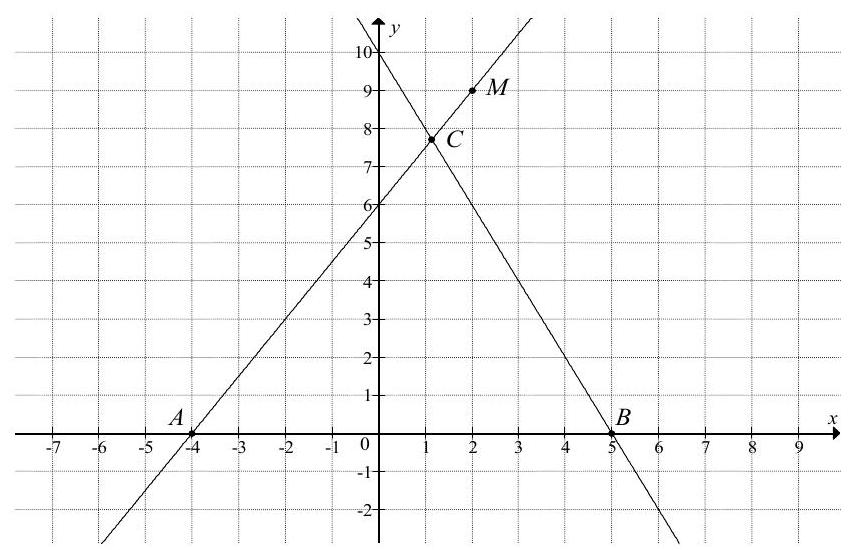
\includegraphics[max width=\textwidth]{2025_02_07_e35f706dbfcfb4be75cfg-17}
\end{center}

Prosta $A M$ przechodzi przez punkty $A=(-4,0)$ i $M=(2,9)$, więc jej równanie ma postać

$$
y=\frac{9}{2+4}(x+4), \text { czyli } y=\frac{3}{2} x+6 .
$$

Prosta $k$ o równaniu $y=-2 x+10$ przecina oś $O x$ w punkcie $B$, więc $B=(5,0)$.\\
Zatem $|A B|=|5-(-4)|=9$.\\
Współrzędne punktu $C$ obliczymy, rozwiązując układ równań:

$$
y=\frac{3}{2} x+6 \text { i } y=-2 x+10
$$

Stąd

$$
\begin{gathered}
\frac{3}{2} x+6=-2 x+10, \\
\frac{7}{2} x=4, \\
x=\frac{8}{7}, \text { a } y=\frac{3}{2} \cdot \frac{8}{7}+6=\frac{12}{7}+6=\frac{54}{7}
\end{gathered}
$$

Zatem $C=\left(\frac{8}{7}, \frac{54}{7}\right)$. Wynika stąd, że wysokość $h$ trójkąta $A B C$ opuszczona z wierzchołka $C$ na podstawę $A B$ jest równa $h=y_{C}=\frac{54}{7}$.\\
Zatem pole trójkąta $A B C$ jest równe

$$
P_{A B C}=\frac{1}{2} \cdot|A B| \cdot h=\frac{1}{2} \cdot 9 \cdot \frac{54}{7}=\frac{243}{7}=34 \frac{5}{7} .
$$

\section*{II sposób}
\begin{center}
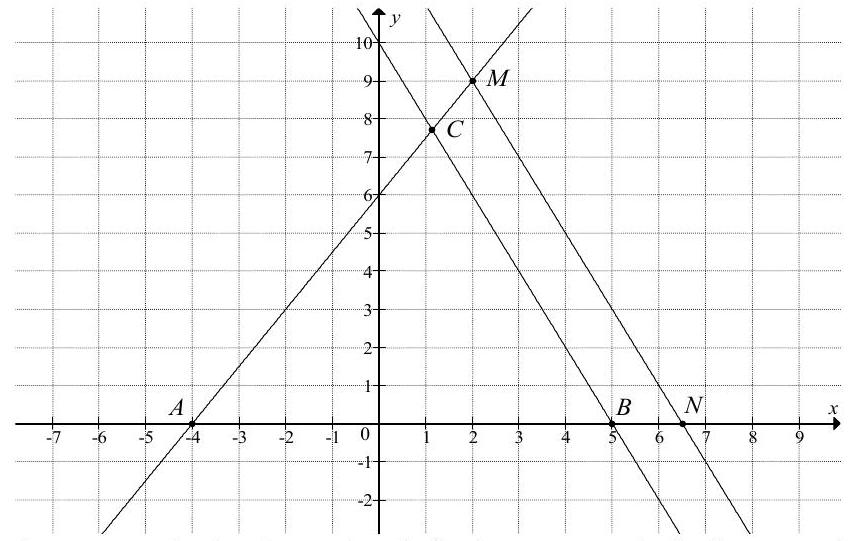
\includegraphics[max width=\textwidth]{2025_02_07_e35f706dbfcfb4be75cfg-18}
\end{center}

Wyznaczamy równanie prostej $l$ równoległej do prostej $k$ i przechodzącej przez punkt $M=(2,9)$ :

$$
\begin{gathered}
y=-2(x-2)+9 \\
y=-2 x+13
\end{gathered}
$$

Niech $N$ będzie punktem przecięcia prostej $l$ z osią $O x$, więc $N=\left(\frac{13}{2}, 0\right)$. Zatem

$$
|A N|=\left|\frac{13}{2}-(-4)\right|=\frac{21}{2} .
$$

Prosta $k$ o równaniu $y=-2 x+10$ przecina oś $O x$ w punkcie $B$, więc $B=(5,0)$.\\
Zatem $|A B|=|5-(-4)|=9$.\\
Z równoległości prostych $k$ i $l$ wynika, że trójkąt $A B C$ jest podobny do trójkąta $A N M$, a skala tego podobieństwa jest równa

$$
s=\frac{|A B|}{|A N|}=\frac{9}{\frac{21}{2}}=\frac{18}{21}=\frac{6}{7} .
$$

Pole trójkąta $A N M$ jest równe

$$
P_{A N M}=\frac{1}{2}|A N| \cdot 9=\frac{1}{2} \cdot \frac{21}{2} \cdot 9=\frac{21 \cdot 9}{4},
$$

więc pole trójkąta $A B C$ jest równe

$$
P_{A B C}=s^{2} \cdot P_{A N M}=\left(\frac{6}{7}\right)^{2} \cdot \frac{21 \cdot 9}{4}=\frac{243}{7}=34 \frac{5}{7} .
$$

\section*{Uwaga}
Mając obliczone współrzędne wierzchołków trójkąta, możemy obliczyć jego pole, korzystając ze wzoru $P_{A B C}=\frac{1}{2} \cdot\left|\left(x_{B}-x_{A}\right)\left(y_{C}-y_{A}\right)-\left(y_{B}-y_{A}\right)\left(x_{C}-x_{A}\right)\right|$ :

$$
P_{A B C}=\frac{1}{2} \cdot\left|(5+4)\left(\frac{54}{7}-0\right)-0 \cdot\left(\frac{8}{7}+4\right)\right|=\frac{1}{2} \cdot\left|9 \cdot \frac{54}{7}\right|=\frac{243}{7}=34 \frac{5}{7} .
$$

\section*{III sposób}
\begin{center}
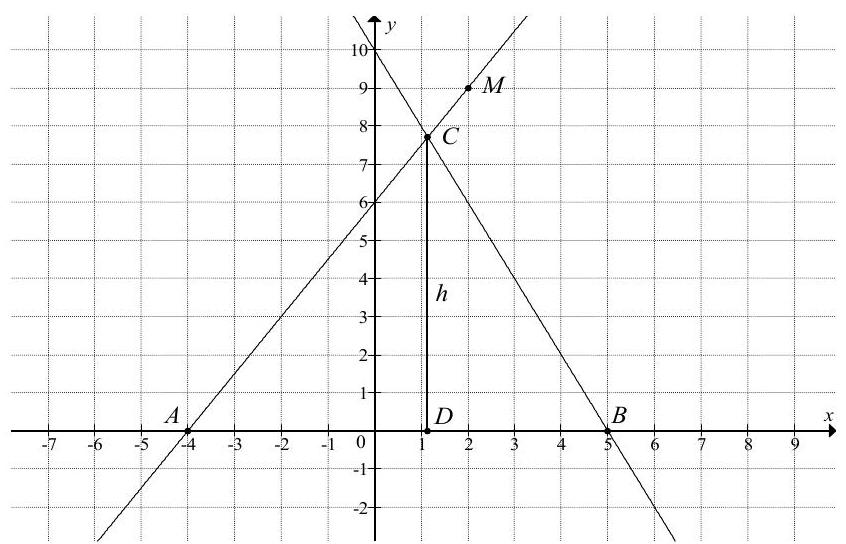
\includegraphics[max width=\textwidth]{2025_02_07_e35f706dbfcfb4be75cfg-19}
\end{center}

Prosta $k$ o równaniu $y=-2 x+10$ przecina oś $O x$ w punkcie $B$, więc $B=(5,0)$.\\
Zatem $|A B|=|5-(-4)|=9$.\\
Niech $h=|C D|$. Ponieważ współczynnik kierunkowy prostej $k$ jest równy -2 , więc

$$
|D A|=\frac{1}{2} h .
$$

Zatem $|A D|=9-\frac{1}{2} h$.\\
Współczynnik kierunkowy prostej $A M$ jest równy $a_{A M}=\frac{9-0}{2-(-4)}=\frac{3}{2}$, ale $a_{A M}=\frac{|C D|}{|A D|}$, więc

$$
\begin{gathered}
\frac{|C D|}{|A D|}=\frac{3}{2}, \\
\frac{h}{9-\frac{1}{2} h}=\frac{3}{2}, \\
2 h=27-\frac{3}{2} h, \\
\frac{7}{2} h=27, \\
h=\frac{54}{7} .
\end{gathered}
$$

Pole trójkąta $A B C$ jest równe

$$
P_{A B C}=\frac{1}{2} \cdot|A B| \cdot h=\frac{1}{2} \cdot 9 \cdot \frac{54}{7}=\frac{243}{7}=34 \frac{5}{7} .
$$

\section*{Schemat punktowania}
Rozwiązanie, w którym postęp jest niewielki, ale konieczny na drodze do pełnego rozwiązania\\
Zdający

\begin{itemize}
  \item wyznaczy współczynnik kierunkowy prostej $A M: a=\frac{3}{2}$\\
albo
  \item wyznaczy współrzędne punktu $B: B=(5,0)$\\
i na tym poprzestanie lub dalej popełnia błędy.\\
Rozwiązanie, w którym postęp jest istotny 2 p.\\
Zdający
  \item zapisze równanie prostej $A M: y=\frac{3}{2} x+6$\\
albo
  \item wyznaczy równanie prostej $M N: y=-2 x+13$ i zapisze, że trójkąty $A B C$ i $A N M$ są podobne,\\
albo
  \item zapisze zależność między długościami odcinków $C D$ i $D A: \frac{|C D|}{|A D|}=\frac{3}{2}$\\
i na tym poprzestanie lub dalej popełnia błędy.\\
Pokonanie zasadniczych trudności zadania 3 p. Zdający
  \item obliczy długość podstawy $A B$ trójkąta: $|A B|=9$ oraz zapisze równanie, z którego można wyznaczyć jedną ze współrzędnych punktu $C$\\
albo
  \item obliczy współrzędne wierzchołka $C: C=\left(\frac{8}{7}, \frac{54}{7}\right)$ (lub drugą współłzzędną tego punktu) i nie zapisze współrzędnych punktu $B$,\\
albo
  \item obliczy skalę podobieństwa trójkąta $A B C$ do trójkąta $A N M: s=\frac{6}{7}$ (lub skalę podobieństwa trójkąta $A N M$ do trójkąta $A B C: s_{1}=\frac{7}{6}$ ),\\
albo
  \item obliczy pole trójkąta $A N M: P_{A N M}=\frac{1}{2} \cdot \frac{21}{2} \cdot 9$ i zapisze, że $P_{A B C}=s^{2} \cdot P_{A N M}$, gdzie $s$ oznacza skalę podobieństwa trójkąta $A B C$ do trójkąta $A N M$,\\
albo
  \item zapisze równanie z jedną niewiadomą, z którego można obliczyć wysokość trójkąta $A B C, \mathrm{np} .: \frac{h}{9-\frac{1}{2} h}=\frac{3}{2}$\\
i na tym poprzestanie lub dalej popełnia błędy.
\end{itemize}

\section*{Rozwiązanie prawie pełne}
\section*{Zdający}
\begin{itemize}
  \item obliczy drugą współrzędną wierzchołka $C$ oraz długość podstawy $A B$ trójkąta $A B C$ : $y_{C}=\frac{54}{7},|A B|=9$\\
albo
  \item obliczy współrzędne wierzchołków $B$ i $C: B=(5,0), C=\left(\frac{8}{7}, \frac{54}{7}\right)$,\\
albo
  \item obliczy skalę podobieństwa trójkąta $A B C$ do trójkąta $A N M: s=\frac{6}{7}$ (lub skalę podobieństwa trójkąta $A N M$ do trójkąta $A B C: s_{1}=\frac{7}{6}$ ) oraz pole trójkąta $A N M$ : $P_{A N M}=\frac{1}{2} \cdot \frac{21}{2} \cdot 9$ i zapisze, że $P_{A B C}=s^{2} \cdot P_{A N M}$,\\
albo
  \item obliczy wysokość $C D$ trójkąta $A B C: h=\frac{54}{7}$\\
i na tym poprzestanie lub dalej popełnia błędy.\\
Rozwiązanie pełne\\
Zdający obliczy pole trójkąta $A B C: P_{A B C}=\frac{243}{7}$.
\end{itemize}

\section*{Uwaga}
Akceptujemy, jeżeli zdający poda pole trójkąta w przybliżeniu, np. 34,714.

Zadanie 33. (0-2)

\begin{center}
\begin{tabular}{|l|l|}
\hline
\begin{tabular}{l}
III. Modelowanie \\
matematyczne. \\
\end{tabular} & \begin{tabular}{l}
10. Elementy statystyki opisowej. Teoria prawdopodobieństwa \\
i kombinatoryka. Zdający oblicza prawdopodobieństwa \\
w prostych sytuacjach, stosując klasyczną definicję \\
prawdopodobieństwa (10.3). \\
\end{tabular} \\
\hline
\end{tabular}
\end{center}

\section*{Przykładowe rozwiązanie}
Jest to model klasyczny i liczba wszystkich zdarzeń elementarnych jest równa $|\Omega|=90$.\\
Zbiór wszystkich zdarzeń elementarnych to zbiór wszystkich liczb naturalnych dwucyfrowych.\\
Niech $A$ oznacza zdarzenie polegające na tym, że wylosujemy liczbę, która jest równocześnie mniejsza od 40 i podzielna przez 3. Zdarzeniu $A$ sprzyjają następujące zdarzenia elementarne

$$
A=\{12,15,18,21,24,27,30,33,36,39\} .
$$

Stąd $|A|=10$.\\
Prawdopodobieństwo zdarzenia $A$ jest równe

$$
P(A)=\frac{|A|}{|\Omega|}=\frac{10}{90}=\frac{1}{9} .
$$

Odpowiedź: Prawdopodobieństwo zdarzenia, polegającego na tym, że wylosujemy liczbę, która jest równocześnie mniejsza od 40 i podzielna przez 3, jest równe $\frac{1}{9}$.

\section*{Schemat punktowania}
Zdający otrzymuje\\
gdy

\begin{itemize}
  \item zapisze, że $|\Omega|=90$\\
albo
  \item zapisze, że $|A|=10$ i nie wskazuje przy tym niepoprawnych zdarzeń elementarnych albo
  \item wypisze wszystkie zdarzenia elementarne sprzyjające zdarzeniu $A$ :
\end{itemize}

$$
12,15,18,21,24,27,30,33,36,39
$$

i na tym poprzestanie lub dalej popełni błędy.\\
Zdający otrzymuje\\
gdy obliczy prawdopodobieństwo zdarzenia $A$ i wynik zapisze w postaci ułamka:\\
$P(A)=\frac{|A|}{|\Omega|}=\frac{10}{90}=\frac{1}{9}$.

\section*{Uwaga}
\begin{enumerate}
  \item Jeżeli zdający błędnie zapisze wynik $P(A)$ jako liczbę większą od 1 lub mniejszą od 0 , to otrzymuje $\mathbf{0}$ punktów za całe rozwiązanie.
  \item Jeżeli w przedstawionym rozwiązaniu zdający interpretuje zdarzenie elementarne jako rezultat wylosowania więcej niż jednej liczby, to za całe rozwiązanie otrzymuje 0 punktów.
  \item Jeżeli zdający w rozwiązaniu zapisze tylko $\frac{1}{9}$, to otrzymuje $\mathbf{0}$ punktów.
\end{enumerate}

Zadanie 34. (0-4)

\begin{center}
\begin{tabular}{|l|l|}
\hline
 & \begin{tabular}{l}
9. Stereometria. Zdający rozpoznaje w graniastosłupach \\
i ostrosłupach kąty między odcinkami (np. krawędziami, \\
krawędziami i przekątnymi. (9.1) \\
Zdajacy rozpoznaje w graniastosłupach i ostrosłupach kąt \\
\end{tabular} \\
IV. Użycie i tworzenie &  \\
strategii. & \begin{tabular}{l}
między odcinkami i płaszczyznami (między krawędziami \\
i ścianami, przekątnymi i ścianami (9.2) \\
Zdający rozpoznaje w graniastosłupach i ostrosłupach kąty \\
między ścianami (9.4) \\
Zdający stosuje trygonometrię do obliczeń długości odcinków, \\
miar kątów, pól powierzchni i objętości (9.6). \\
\end{tabular} \\
\hline
\end{tabular}
\end{center}

\section*{Przykładowe rozwiązanie}
Przyjmijmy oznaczenia jak na rysunku.\\
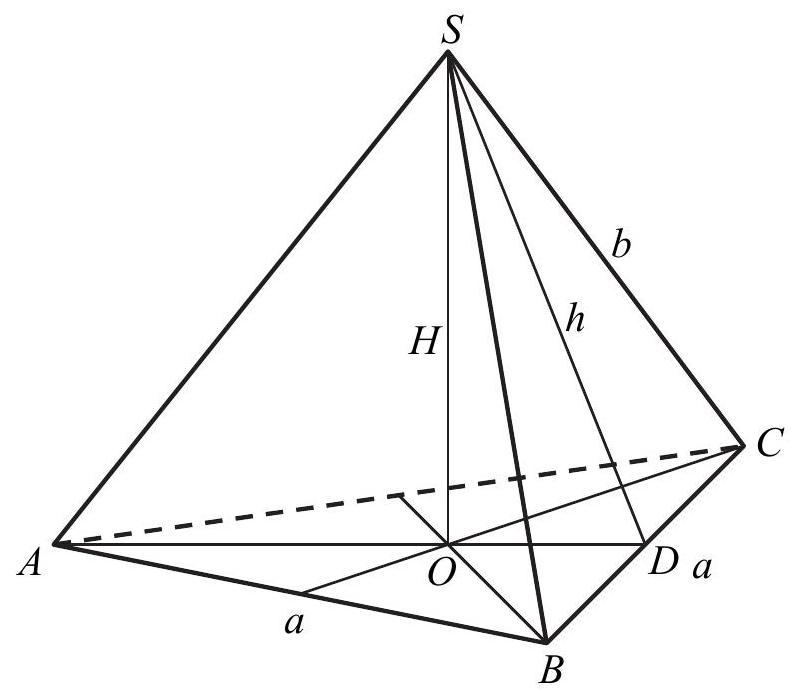
\includegraphics[max width=\textwidth, center]{2025_02_07_e35f706dbfcfb4be75cfg-23}

Wykorzystujemy wzór na pole powierzchni bocznej ostrosłupa i zapisujemy równanie

$$
\frac{15 \sqrt{3}}{4}=3 \cdot \frac{1}{2} a \cdot \frac{5 \sqrt{3}}{4}, \text { skąd otrzymujemy } a=2 .
$$

Z twierdzenia Pitagorasa dla trójkąta $D O S$ otrzymujemy

$$
H^{2}=h^{2}-|D O|^{2}
$$

Ponieważ $|D O|=\frac{1}{3} a \cdot \frac{\sqrt{3}}{2}=\frac{\sqrt{3}}{3}$, więc

$$
H^{2}=\left(\frac{5 \sqrt{3}}{4}\right)^{2}-\left(\frac{\sqrt{3}}{3}\right)^{2}
$$

Stąd $H=\frac{\sqrt{209}}{4 \sqrt{3}}$.\\
Zatem objętość ostrosłupa jest równa

$$
V=\frac{1}{3} P_{p} \cdot H=\frac{1}{3} \cdot \frac{4 \sqrt{3}}{4} \cdot \frac{\sqrt{209}}{4 \sqrt{3}}=\frac{\sqrt{209}}{12} .
$$

\section*{Schemat punktowania}
Rozwiązanie, w którym postęp jest wprawdzie niewielki, ale konieczny na drodze do pełnego rozwiązania zadania\\
Zdający

\begin{itemize}
  \item zapisze równanie $\frac{15 \sqrt{3}}{4}=3 \cdot \frac{1}{2} a \cdot \frac{5 \sqrt{3}}{4}$\\
albo
  \item zapisze, że $|D O|=\frac{1}{3} a \cdot \frac{\sqrt{3}}{2}$ lub $|A O|=\frac{2}{3} a \cdot \frac{\sqrt{3}}{2}$\\
i na tym zakończy lub dalej popełnia błędy.\\
Rozwiązanie, w którym postęp jest istotny 2 p. Zdający
  \item obliczy długość krawędzi $a$ podstawy ostrosłupa: $a=2$ i zapisze równanie z niewiadomą $H$, np.: $H^{2}=\left(\frac{5 \sqrt{3}}{4}\right)^{2}-\left(\frac{a \sqrt{3}}{6}\right)^{2}$\\
albo
  \item obliczy długość krawędzi $a$ podstawy ostrosłupa: $a=2$ i zapisze układ równań wystarczający do obliczenia wysokości ostrosłupa, np.: $\left\{\begin{array}{l}H^{2}+\left(\frac{a \sqrt{3}}{3}\right)^{2}=b^{2} \\ \left(\frac{a}{2}\right)^{2}+\left(\frac{5 \sqrt{3}}{4}\right)^{2}=b^{2}\end{array}\right.$ i na tym zakończy lub dalej popełnia błędy.\\
Pokonanie zasadniczych trudności zadania\\
Zdający obliczy wysokość ostrosłupa: $H=\frac{\sqrt{209}}{4 \sqrt{3}}$ i na tym zakończy lub dalej popełnia błędy.\\
Rozwiązanie pełne 4 p.\\
Zdający obliczy objętość $V$ ostrosłupa: $V=\frac{\sqrt{209}}{12}$.
\end{itemize}

\section*{Uwagi}
\begin{enumerate}
  \item Jeżeli zdający rozważa inną bryłę niż podana w treści zadania, to otrzymuje $\mathbf{0}$ punktów.
  \item Akceptujemy poprawne przybliżenia liczb rzeczywistych.
  \item Jeżeli zdający poda długość krawędzi podstawy $a=2$ bez obliczeń i rozwiąże zadanie do końca, to otrzymuje co najwyżej $\mathbf{3}$ punkty.
  \item Jeżeli zdający błędnie przepisze liczbę $\frac{5 \sqrt{3}}{4}$ lub liczbę $\frac{15 \sqrt{3}}{4}$ i z tym błędem rozwiąże zadanie konsekwentnie do końca, to otrzymuje co najwyżej $\mathbf{3}$ punkty.
  \item Jeśli zdający nie obliczy $a$ i przyjmuje, że ściany boczne są trójkątami równobocznymi, to otrzymuje $\mathbf{0}$ punktów.
\end{enumerate}

\end{document}